\documentclass[12pt]{article}
\usepackage{tikz}
\usepackage{amsmath}
\usepackage{amsfonts}
\usepackage{geometry}
\usepackage{amssymb}
\usepackage{wasysym}
\usepackage{color}
\usepackage[utf8]{inputenc}
\usepackage{pdfpages}
\usepackage{listings}
\newgeometry{top=1 cm,bottom=2cm,left=0.5cm,right=0.5cm}
\title{ }
\date{}
\author{}


\definecolor{mygreen}{rgb}{0,0.6,0}
\definecolor{mygray}{rgb}{0.5,0.5,0.5}
\definecolor{mymauve}{rgb}{0.58,0,0.82}

\lstset{ %
  backgroundcolor=\color{white},   % choose the background color; you must add \usepackage{color} or \usepackage{xcolor}
  basicstyle=\footnotesize,        % the size of the fonts that are used for the code
  breakatwhitespace=false,         % sets if automatic breaks should only happen at whitespace
  breaklines=true,                 % sets automatic line breaking
  captionpos=b,                    % sets the caption-position to bottom
  commentstyle=\color{mygreen},    % comment style
  deletekeywords={...},            % if you want to delete keywords from the given language
  escapeinside={\%*}{*)},          % if you want to add LaTeX within your code
  extendedchars=true,              % lets you use non-ASCII characters; for 8-bits encodings only, does not work with UTF-8
  frame=single,	                   % adds a frame around the code
  keepspaces=true,                 % keeps spaces in text, useful for keeping indentation of code (possibly needs columns=flexible)
  keywordstyle=\color{blue},       % keyword style
  language=Octave,                 % the language of the code
  otherkeywords={*,...},           % if you want to add more keywords to the set
  numbers=left,                    % where to put the line-numbers; possible values are (none, left, right)
  numbersep=5pt,                   % how far the line-numbers are from the code
  numberstyle=\tiny\color{mygray}, % the style that is used for the line-numbers
  rulecolor=\color{black},         % if not set, the frame-color may be changed on line-breaks within not-black text (e.g. comments (green here))
  showspaces=false,                % show spaces everywhere adding particular underscores; it overrides 'showstringspaces'
  showstringspaces=false,          % underline spaces within strings only
  showtabs=false,                  % show tabs within strings adding particular underscores
  stepnumber=2,                    % the step between two line-numbers. If it's 1, each line will be numbered
  stringstyle=\color{mymauve},     % string literal style
  tabsize=2,	                   % sets default tabsize to 2 spaces
  title=\lstname,                  % show the filename of files included with \lstinputlisting; also try caption instead of title
  xleftmargin=0cm,
}

\title{}
\date{}
\author{}
\begin{document}

\vbox{
\noindent la gráfica de linea de $K_5$ (hipereneŕgética por vértices)\\
Total energy: 20 \\\ 
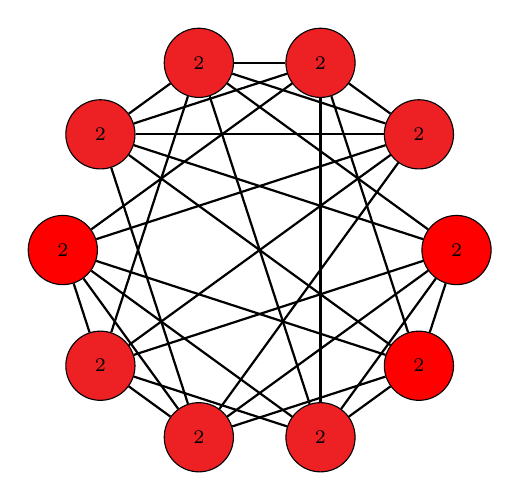
\begin{tikzpicture}
\node[style={circle,fill=yellow!1!red!99,draw,minimum size=2.5em,inner sep=3pt]}] (1) at (1*360/10:2.5) {$\scriptstyle{2}$};
\node[style={circle,fill=yellow!1!red!99,draw,minimum size=2.5em,inner sep=3pt]}] (2) at (2*360/10:2.5) {$\scriptstyle{2}$};
\node[style={circle,fill=yellow!1!red!99,draw,minimum size=2.5em,inner sep=3pt]}] (3) at (3*360/10:2.5) {$\scriptstyle{2}$};
\node[style={circle,fill=yellow!1!red!99,draw,minimum size=2.5em,inner sep=3pt]}] (4) at (4*360/10:2.5) {$\scriptstyle{2}$};
\node[style={circle,fill=yellow!0!red!100,draw,minimum size=2.5em,inner sep=3pt]}] (5) at (5*360/10:2.5) {$\scriptstyle{2}$};
\node[style={circle,fill=yellow!1!red!99,draw,minimum size=2.5em,inner sep=3pt]}] (6) at (6*360/10:2.5) {$\scriptstyle{2}$};
\node[style={circle,fill=yellow!1!red!99,draw,minimum size=2.5em,inner sep=3pt]}] (7) at (7*360/10:2.5) {$\scriptstyle{2}$};
\node[style={circle,fill=yellow!1!red!99,draw,minimum size=2.5em,inner sep=3pt]}] (8) at (8*360/10:2.5) {$\scriptstyle{2}$};
\node[style={circle,fill=yellow!0!red!100,draw,minimum size=2.5em,inner sep=3pt]}] (9) at (9*360/10:2.5) {$\scriptstyle{2}$};
\node[style={circle,fill=yellow!0!red!100,draw,minimum size=2.5em,inner sep=3pt]}] (10) at (10*360/10:2.5) {$\scriptstyle{2}$};
\path[draw,thick](1) edge node {} (2);
\path[draw,thick](1) edge node {} (3);
\path[draw,thick](1) edge node {} (4);
\path[draw,thick](1) edge node {} (5);
\path[draw,thick](1) edge node {} (6);
\path[draw,thick](1) edge node {} (7);
\path[draw,thick](2) edge node {} (3);
\path[draw,thick](2) edge node {} (4);
\path[draw,thick](2) edge node {} (5);
\path[draw,thick](2) edge node {} (8);
\path[draw,thick](2) edge node {} (9);
\path[draw,thick](3) edge node {} (4);
\path[draw,thick](3) edge node {} (6);
\path[draw,thick](3) edge node {} (8);
\path[draw,thick](3) edge node {} (10);
\path[draw,thick](4) edge node {} (7);
\path[draw,thick](4) edge node {} (9);
\path[draw,thick](4) edge node {} (10);
\path[draw,thick](5) edge node {} (6);
\path[draw,thick](5) edge node {} (7);
\path[draw,thick](5) edge node {} (8);
\path[draw,thick](5) edge node {} (9);
\path[draw,thick](6) edge node {} (7);
\path[draw,thick](6) edge node {} (8);
\path[draw,thick](6) edge node {} (10);
\path[draw,thick](7) edge node {} (9);
\path[draw,thick](7) edge node {} (10);
\path[draw,thick](8) edge node {} (9);
\path[draw,thick](8) edge node {} (10);
\path[draw,thick](9) edge node {} (10);
\end{tikzpicture}
\\}


\vbox{

\noindent $K_{10}$\\

Total energy: 18 \\\ 
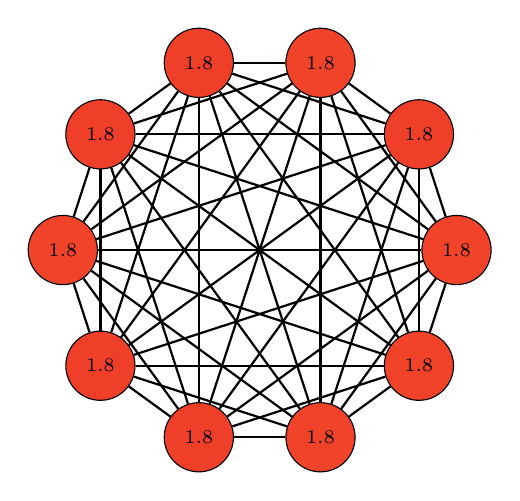
\begin{tikzpicture}
\node[style={circle,fill=yellow!10!red!92,draw,minimum size=2.5em,inner sep=3pt]}] (1) at (1*360/10:2.5) {$\scriptstyle{1.8}$};
\node[style={circle,fill=yellow!11!red!91,draw,minimum size=2.5em,inner sep=3pt]}] (2) at (2*360/10:2.5) {$\scriptstyle{1.8}$};
\node[style={circle,fill=yellow!10!red!92,draw,minimum size=2.5em,inner sep=3pt]}] (3) at (3*360/10:2.5) {$\scriptstyle{1.8}$};
\node[style={circle,fill=yellow!10!red!92,draw,minimum size=2.5em,inner sep=3pt]}] (4) at (4*360/10:2.5) {$\scriptstyle{1.8}$};
\node[style={circle,fill=yellow!11!red!91,draw,minimum size=2.5em,inner sep=3pt]}] (5) at (5*360/10:2.5) {$\scriptstyle{1.8}$};
\node[style={circle,fill=yellow!10!red!92,draw,minimum size=2.5em,inner sep=3pt]}] (6) at (6*360/10:2.5) {$\scriptstyle{1.8}$};
\node[style={circle,fill=yellow!10!red!92,draw,minimum size=2.5em,inner sep=3pt]}] (7) at (7*360/10:2.5) {$\scriptstyle{1.8}$};
\node[style={circle,fill=yellow!11!red!91,draw,minimum size=2.5em,inner sep=3pt]}] (8) at (8*360/10:2.5) {$\scriptstyle{1.8}$};
\node[style={circle,fill=yellow!11!red!91,draw,minimum size=2.5em,inner sep=3pt]}] (9) at (9*360/10:2.5) {$\scriptstyle{1.8}$};
\node[style={circle,fill=yellow!11!red!91,draw,minimum size=2.5em,inner sep=3pt]}] (10) at (10*360/10:2.5) {$\scriptstyle{1.8}$};
\path[draw,thick](1) edge node {} (2);
\path[draw,thick](1) edge node {} (3);
\path[draw,thick](1) edge node {} (4);
\path[draw,thick](1) edge node {} (5);
\path[draw,thick](1) edge node {} (6);
\path[draw,thick](1) edge node {} (7);
\path[draw,thick](1) edge node {} (8);
\path[draw,thick](1) edge node {} (9);
\path[draw,thick](1) edge node {} (10);
\path[draw,thick](2) edge node {} (3);
\path[draw,thick](2) edge node {} (4);
\path[draw,thick](2) edge node {} (5);
\path[draw,thick](2) edge node {} (6);
\path[draw,thick](2) edge node {} (7);
\path[draw,thick](2) edge node {} (8);
\path[draw,thick](2) edge node {} (9);
\path[draw,thick](2) edge node {} (10);
\path[draw,thick](3) edge node {} (4);
\path[draw,thick](3) edge node {} (5);
\path[draw,thick](3) edge node {} (6);
\path[draw,thick](3) edge node {} (7);
\path[draw,thick](3) edge node {} (8);
\path[draw,thick](3) edge node {} (9);
\path[draw,thick](3) edge node {} (10);
\path[draw,thick](4) edge node {} (5);
\path[draw,thick](4) edge node {} (6);
\path[draw,thick](4) edge node {} (7);
\path[draw,thick](4) edge node {} (8);
\path[draw,thick](4) edge node {} (9);
\path[draw,thick](4) edge node {} (10);
\path[draw,thick](5) edge node {} (6);
\path[draw,thick](5) edge node {} (7);
\path[draw,thick](5) edge node {} (8);
\path[draw,thick](5) edge node {} (9);
\path[draw,thick](5) edge node {} (10);
\path[draw,thick](6) edge node {} (7);
\path[draw,thick](6) edge node {} (8);
\path[draw,thick](6) edge node {} (9);
\path[draw,thick](6) edge node {} (10);
\path[draw,thick](7) edge node {} (8);
\path[draw,thick](7) edge node {} (9);
\path[draw,thick](7) edge node {} (10);
\path[draw,thick](8) edge node {} (9);
\path[draw,thick](8) edge node {} (10);
\path[draw,thick](9) edge node {} (10);
\end{tikzpicture}
\\}


\vbox{

\noindent gráfica obtenida añadiento una hoja a la gráfica de linea de $K_5$ (hiperenergética pero no por vértice)\\

Total energy: 20.7 \\\ 
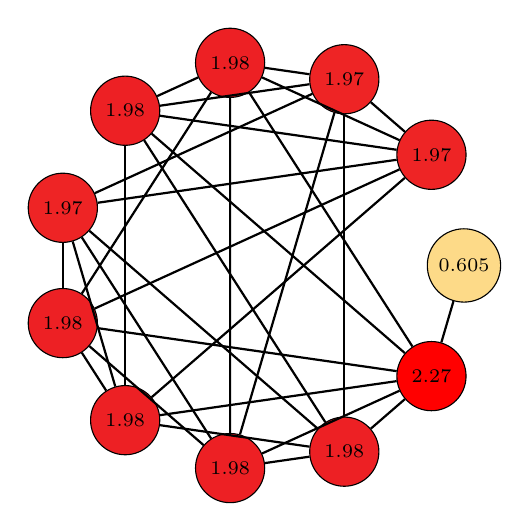
\begin{tikzpicture}
\node[style={circle,fill=yellow!2!red!98,draw,minimum size=2.5em,inner sep=3pt]}] (1) at (1*360/11:2.6) {$\scriptstyle{1.97}$};
\node[style={circle,fill=yellow!2!red!98,draw,minimum size=2.5em,inner sep=3pt]}] (2) at (2*360/11:2.6) {$\scriptstyle{1.97}$};
\node[style={circle,fill=yellow!1!red!99,draw,minimum size=2.5em,inner sep=3pt]}] (3) at (3*360/11:2.6) {$\scriptstyle{1.98}$};
\node[style={circle,fill=yellow!1!red!99,draw,minimum size=2.5em,inner sep=3pt]}] (4) at (4*360/11:2.6) {$\scriptstyle{1.98}$};
\node[style={circle,fill=yellow!2!red!98,draw,minimum size=2.5em,inner sep=3pt]}] (5) at (5*360/11:2.6) {$\scriptstyle{1.97}$};
\node[style={circle,fill=yellow!1!red!99,draw,minimum size=2.5em,inner sep=3pt]}] (6) at (6*360/11:2.6) {$\scriptstyle{1.98}$};
\node[style={circle,fill=yellow!1!red!99,draw,minimum size=2.5em,inner sep=3pt]}] (7) at (7*360/11:2.6) {$\scriptstyle{1.98}$};
\node[style={circle,fill=yellow!1!red!99,draw,minimum size=2.5em,inner sep=3pt]}] (8) at (8*360/11:2.6) {$\scriptstyle{1.98}$};
\node[style={circle,fill=yellow!1!red!99,draw,minimum size=2.5em,inner sep=3pt]}] (9) at (9*360/11:2.6) {$\scriptstyle{1.98}$};
\node[style={circle,fill=yellow!0!red!100,draw,minimum size=2.5em,inner sep=3pt]}] (10) at (10*360/11:2.6) {$\scriptstyle{2.27}$};
\node[style={circle,fill=yellow!70!red!44,draw,minimum size=2.5em,inner sep=3pt]}] (11) at (11*360/11:2.6) {$\scriptstyle{0.605}$};
\path[draw,thick](1) edge node {} (2);
\path[draw,thick](1) edge node {} (3);
\path[draw,thick](1) edge node {} (4);
\path[draw,thick](1) edge node {} (5);
\path[draw,thick](1) edge node {} (6);
\path[draw,thick](1) edge node {} (7);
\path[draw,thick](2) edge node {} (3);
\path[draw,thick](2) edge node {} (4);
\path[draw,thick](2) edge node {} (5);
\path[draw,thick](2) edge node {} (8);
\path[draw,thick](2) edge node {} (9);
\path[draw,thick](3) edge node {} (4);
\path[draw,thick](3) edge node {} (6);
\path[draw,thick](3) edge node {} (8);
\path[draw,thick](3) edge node {} (10);
\path[draw,thick](4) edge node {} (7);
\path[draw,thick](4) edge node {} (9);
\path[draw,thick](4) edge node {} (10);
\path[draw,thick](5) edge node {} (6);
\path[draw,thick](5) edge node {} (7);
\path[draw,thick](5) edge node {} (8);
\path[draw,thick](5) edge node {} (9);
\path[draw,thick](6) edge node {} (7);
\path[draw,thick](6) edge node {} (8);
\path[draw,thick](6) edge node {} (10);
\path[draw,thick](7) edge node {} (9);
\path[draw,thick](7) edge node {} (10);
\path[draw,thick](8) edge node {} (9);
\path[draw,thick](8) edge node {} (10);
\path[draw,thick](9) edge node {} (10);
\path[draw,thick](10) edge node {} (11);
\end{tikzpicture}
\\}

\vbox{

\noindent $K_{11}$\\

Total energy: 20 \\\ 
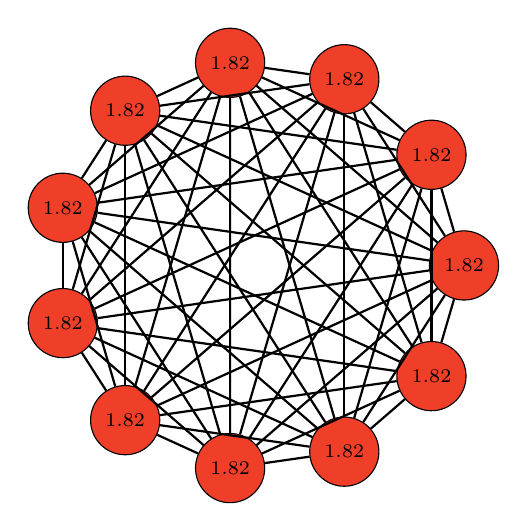
\begin{tikzpicture}
\node[style={circle,fill=yellow!10!red!92,draw,minimum size=2.5em,inner sep=3pt]}] (1) at (1*360/11:2.6) {$\scriptstyle{1.82}$};
\node[style={circle,fill=yellow!10!red!92,draw,minimum size=2.5em,inner sep=3pt]}] (2) at (2*360/11:2.6) {$\scriptstyle{1.82}$};
\node[style={circle,fill=yellow!10!red!92,draw,minimum size=2.5em,inner sep=3pt]}] (3) at (3*360/11:2.6) {$\scriptstyle{1.82}$};
\node[style={circle,fill=yellow!10!red!92,draw,minimum size=2.5em,inner sep=3pt]}] (4) at (4*360/11:2.6) {$\scriptstyle{1.82}$};
\node[style={circle,fill=yellow!10!red!92,draw,minimum size=2.5em,inner sep=3pt]}] (5) at (5*360/11:2.6) {$\scriptstyle{1.82}$};
\node[style={circle,fill=yellow!10!red!92,draw,minimum size=2.5em,inner sep=3pt]}] (6) at (6*360/11:2.6) {$\scriptstyle{1.82}$};
\node[style={circle,fill=yellow!10!red!92,draw,minimum size=2.5em,inner sep=3pt]}] (7) at (7*360/11:2.6) {$\scriptstyle{1.82}$};
\node[style={circle,fill=yellow!10!red!92,draw,minimum size=2.5em,inner sep=3pt]}] (8) at (8*360/11:2.6) {$\scriptstyle{1.82}$};
\node[style={circle,fill=yellow!10!red!92,draw,minimum size=2.5em,inner sep=3pt]}] (9) at (9*360/11:2.6) {$\scriptstyle{1.82}$};
\node[style={circle,fill=yellow!10!red!92,draw,minimum size=2.5em,inner sep=3pt]}] (10) at (10*360/11:2.6) {$\scriptstyle{1.82}$};
\node[style={circle,fill=yellow!10!red!92,draw,minimum size=2.5em,inner sep=3pt]}] (11) at (11*360/11:2.6) {$\scriptstyle{1.82}$};
\path[draw,thick](1) edge node {} (2);
\path[draw,thick](1) edge node {} (3);
\path[draw,thick](1) edge node {} (4);
\path[draw,thick](1) edge node {} (5);
\path[draw,thick](1) edge node {} (6);
\path[draw,thick](1) edge node {} (7);
\path[draw,thick](1) edge node {} (8);
\path[draw,thick](1) edge node {} (9);
\path[draw,thick](1) edge node {} (10);
\path[draw,thick](1) edge node {} (11);
\path[draw,thick](2) edge node {} (3);
\path[draw,thick](2) edge node {} (4);
\path[draw,thick](2) edge node {} (5);
\path[draw,thick](2) edge node {} (6);
\path[draw,thick](2) edge node {} (7);
\path[draw,thick](2) edge node {} (8);
\path[draw,thick](2) edge node {} (9);
\path[draw,thick](2) edge node {} (10);
\path[draw,thick](2) edge node {} (11);
\path[draw,thick](3) edge node {} (4);
\path[draw,thick](3) edge node {} (5);
\path[draw,thick](3) edge node {} (6);
\path[draw,thick](3) edge node {} (7);
\path[draw,thick](3) edge node {} (8);
\path[draw,thick](3) edge node {} (9);
\path[draw,thick](3) edge node {} (10);
\path[draw,thick](3) edge node {} (11);
\path[draw,thick](4) edge node {} (5);
\path[draw,thick](4) edge node {} (6);
\path[draw,thick](4) edge node {} (7);
\path[draw,thick](4) edge node {} (8);
\path[draw,thick](4) edge node {} (9);
\path[draw,thick](4) edge node {} (10);
\path[draw,thick](4) edge node {} (11);
\path[draw,thick](5) edge node {} (6);
\path[draw,thick](5) edge node {} (7);
\path[draw,thick](5) edge node {} (8);
\path[draw,thick](5) edge node {} (9);
\path[draw,thick](5) edge node {} (10);
\path[draw,thick](5) edge node {} (11);
\path[draw,thick](6) edge node {} (7);
\path[draw,thick](6) edge node {} (8);
\path[draw,thick](6) edge node {} (9);
\path[draw,thick](6) edge node {} (10);
\path[draw,thick](6) edge node {} (11);
\path[draw,thick](7) edge node {} (8);
\path[draw,thick](7) edge node {} (9);
\path[draw,thick](7) edge node {} (10);
\path[draw,thick](7) edge node {} (11);
\path[draw,thick](8) edge node {} (9);
\path[draw,thick](8) edge node {} (10);
\path[draw,thick](8) edge node {} (11);
\path[draw,thick](9) edge node {} (10);
\path[draw,thick](9) edge node {} (11);
\path[draw,thick](10) edge node {} (11);
\end{tikzpicture}
\\}










\end{document}